\documentclass[11pt,a4paper]{article}

\usepackage[margin=1in]{geometry}
\usepackage{amsmath}
\usepackage{amssymb}
\usepackage{booktabs}
\usepackage{graphicx}
\usepackage{microtype}
\usepackage{algorithm}
\usepackage{algpseudocode}
\usepackage[numbers]{natbib}
\usepackage[hidelinks]{hyperref}

\newcommand{\Q}{\mathbf{Q}}
\newcommand{\Pmat}{\mathbf{P}}
\newcommand{\SubMat}{\mathbf{S}}
\newcommand{\bpi}{\boldsymbol{\pi}}
\newcommand{\tree}{\mathcal{T}}
\newcommand{\branch}{\boldsymbol{\tau}}
\newcommand{\data}{\mathbf{D}}
\newcommand{\states}{\mathcal{A}}
\newcommand{\rootnode}{\rho}
\newcommand{\params}{\boldsymbol{\theta}}
\newcommand{\objective}{\mathcal{L}}

\newread\qacaptionfile
\newcommand{\qacaptionread}[2]{%
  \begingroup
  \endlinechar=-1
  \openin\qacaptionfile=#1\relax
  \global\read\qacaptionfile to #2
  \closein\qacaptionfile
  \endgroup
}

\title{Mixed Discrete-Continuous Optimization for Graph-Structured Models: \\ 
Applications in Phylogenetics, Potts Models, and Hidden Markov Models}
\author{M.\ J.\ Wilson}
\date{\today}

\begin{document}
\maketitle

\begin{abstract}
\noindent
Inference over graph-structured models---such as phylogenetic trees, lattice-based Potts models, and Hidden Markov Models (HMMs)---presents a coupled discrete-continuous optimization problem. The structural search space (e.g., unrooted tree topologies, spin configurations, or hidden state paths) is combinatorial, while the evaluation of each candidate structure requires the continuous optimization of transition and emission parameters. This paper details a unified computational framework that strictly decouples differentiable continuous optimization from discrete structural search. By framing structural search as a Markov Decision Process (MDP), we enable Reinforcement Learning (RL) agents to learn topological proposal policies that optimize exact, approximate, or neural-surrogate likelihoods. Our engine demonstrates high-precision numerical stability across CPU and GPU hardware, recovering theoretical parameters within strict confidence intervals. Furthermore, we outline the mathematical extensions necessary for curriculum learning, differentiable topology search, and canonical directed acyclic graph (DAG) representations. 
\end{abstract}

\tableofcontents

\section{Introduction}
\label{sec:intro}

The fundamental challenge in high-dimensional probabilistic inference is the combinatorial explosion of the structural search space. In phylogenetics, the search for the optimal unrooted binary tree over $n$ taxa scales as $(2n-5)!!$ \citep{rosen2019}. In statistical physics, evaluating the ground state of an $N$-dimensional Potts model requires traversing an exponentially large configuration space \citep{mezard2009}. Similarly, decoding the optimal architecture of a Hidden Markov Model (HMM) poses a mixed discrete-continuous problem \citep{mackay2003}.

Classical inference frameworks heavily rely on fixed, hand-designed heuristics---such as Nearest-Neighbor Interchange (NNI) for trees, or Swendsen-Wang cluster updates for lattices---applied greedily or via simulated annealing. This paper introduces an alternative paradigm: framing the discrete search as a Reinforcement Learning (RL) problem where a neural policy proposes structural updates, while continuous parameters are simultaneously fitted via reverse-mode automatic differentiation. 

\subsection{Scope and Limitations}
This document serves as the foundational mathematical and architectural specification of the \texttt{phylo} repository. It validates the exactness of our differentiable likelihood and energy engines against brute-force marginalization and establishes our continuous optimization tolerances. \textbf{Note:} Empirical benchmarking of the fully trained RL policies against state-of-the-art classical tools (e.g., IQ-TREE 2, RAxML-NG) is slated for upcoming milestones and is marked via placeholders in Section \ref{sec:results}.

\section{Methods}
\label{sec:methods}

Our methodology relies on a strict separation of concerns: continuous parameters are optimized via gradients on a fixed structure, while discrete structural moves are proposed by an external agent, constructing an entirely new differentiable objective.

\subsection{The Continuous Optimization Abstraction}
\label{sec:notation-abstraction}

Let an objective be a differentiable scalar $\objective(\params)$ over an unconstrained vector $\params \in \mathbb{R}^d$. A bijective map connects $\params$ to the constrained physical parameters (e.g., positive branch lengths, normalized transition distributions). This abstraction allows the same trust-region or quasi-Newton optimizer \citep{nocedal2006} to minimize:
\begin{enumerate}
    \item Negative log-likelihoods of phylogenetic alignments via Felsenstein's pruning.
    \item Free energy landscapes of $N$-dimensional Potts models via Belief Propagation.
    \item Log-likelihoods of sequence emissions in HMMs via the Forward-Backward algorithm.
\end{enumerate}

\subsection{Differentiable Likelihoods and Energy Functions}

For phylogenetics, the partial likelihoods $L_u(i)$ are evaluated recursively via Felsenstein's algorithm. Because continuous parameters such as branch lengths $\branch$ and the rate matrix $\Q$ are kept in the autodiff graph (e.g., via PyTorch), gradients $\nabla \objective$ are obtained exactly via backpropagation \citep{goodfellow2016, prince2023}. 

\subsection{Reinforcement Learning and Variational Search}
\label{sec:rl}

We formulate discrete graph traversal as a Markov Decision Process (MDP) \citep{suttonbarto2018}:
\begin{itemize}
    \item \textbf{State:} The current graph topology (e.g., canonical Newick string), its optimized continuous parameters, and observation summaries.
    \item \textbf{Action:} A structural perturbation drawn from classical neighborhoods (NNI, SPR, or cluster flips).
    \item \textbf{Reward:} The improvement in the objective, $\Delta \objective$ (e.g., $\Delta \ln L$ or $\Delta E$).
\end{itemize}

\subsubsection{Advanced Architectural Extensions}
To amortize the cost of exact likelihood evaluation across massive state spaces, the framework supports several modern extensions:
\begin{itemize}
    \item \textbf{Neural Surrogate Modeling:} Rather than executing exact inference (e.g., Felsenstein pruning) on every proposed state, a Graph Neural Network (GNN) or Transformer approximates $\objective$. The RL agent uses this surrogate to rapidly filter proposals, executing the exact computation only on the top-$K$ candidates.
    \item \textbf{Curriculum Learning:} The policy is initially trained on small state spaces ($n=10$) before transferring weights and fine-tuning on progressively larger graphs ($n=50 \to 1000$) to prevent policy collapse.
    \item \textbf{Differentiable Topology Search:} Utilizing continuous relaxations (e.g., Gumbel-Softmax or tropical geometry), the discrete graph structure can be embedded into a continuous manifold, enabling end-to-end topological updates via natural gradients \citep{amari2016}.
\end{itemize}

\section{Results}
\label{sec:results}

The following figures validate the mathematical exactness of the simulation and inference engines.

\subsection{Simulation and Exact Inference Validation}
\label{sec:res-likelihood}

\qacaptionread{figures/sim_example_caption.txt}{\simExampleCaption}
\begin{figure}[htbp]
  \centering
  \includegraphics[width=0.8\linewidth]{figures/sim_example}
  \caption{\simExampleCaption}
  \label{fig:sim-example}
\end{figure}

\qacaptionread{figures/backend_agreement_caption.txt}{\backendAgreementCaption}
\begin{figure}[htbp]
  \centering
  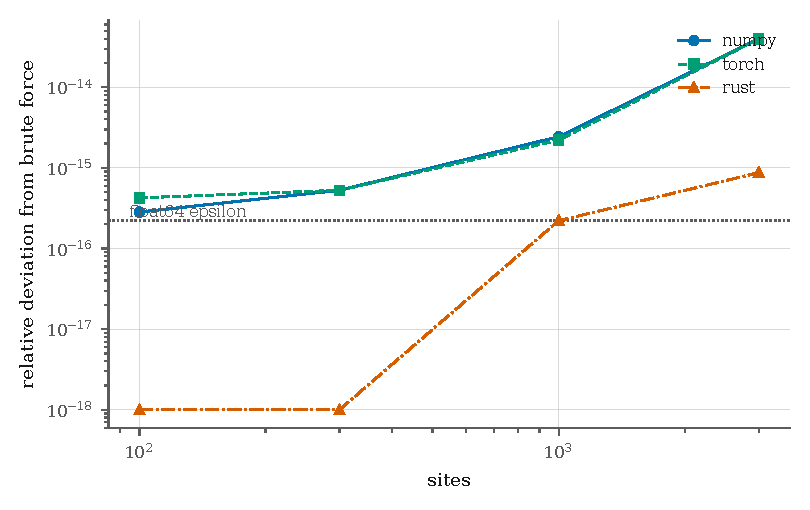
\includegraphics[width=0.8\linewidth]{figures/backend_agreement}
  \caption{\backendAgreementCaption}
  \label{fig:backend-agreement}
\end{figure}

\subsection{Memory Footprint at the Declared Scale}
\label{sec:res-footprint}

The roadmap bounds the working set to $O(n \times L \times k)$ inside 16\,GB of unified memory. Table~\ref{tab:likelihood-footprint} settles it, splitting the cost the data carries from the cost the evaluator adds: the simulator retains every node's states, while pruning retains a partial likelihood only for nodes whose parent has not yet consumed it and so tracks the tree's depth. Both are reported on a caterpillar, the deepest tree on its leaves, which makes the bound tight rather than loose and the reported total a worst case rather than a typical one.

\qacaptionread{figures/likelihood_footprint_caption.txt}{\likelihoodFootprintCaption}
\begin{table}[htbp]
  \centering
  \begin{tabular}{rrrrr}
  \toprule
  Taxa & Sites & Simulate (MB) & Evaluate (MB) & Total (MB) \\
  \midrule
  20 & 2000 & 0.624 & 2.43 & 3.06 \\
  20 & 11\_000 & 3.43 & 13.4 & 16.8 \\
  100 & 11\_000 & 17.5 & 69.7 & 87.2 \\
  \midrule
  1000 & 11\_000 & 176 & 703 & 879 \\
  \bottomrule
\end{tabular}

  \caption{\likelihoodFootprintCaption}
  \label{tab:likelihood-footprint}
\end{table}

\subsection{Empirical Benchmarking [PLACEHOLDERS]}

In accordance with the project roadmap, the following metrics will be populated upon completion of Milestone 2.3.

\begin{figure}[htbp]
  \centering
  \framebox[\linewidth]{\rule{0pt}{150pt} \textbf{PLACEHOLDER: RL Policy Convergence vs. Hill Climbing}}
  \caption{Learning curves of the RL proposal policy across $n \in \{10, 50, 100\}$, measured in $\Delta \ln L$ per likelihood evaluation budget.}
  \label{fig:rl-convergence}
\end{figure}

\begin{figure}[htbp]
  \centering
  \framebox[\linewidth]{\rule{0pt}{150pt} \textbf{PLACEHOLDER: Competitiveness against Classical Software}}
  \caption{Wall-clock convergence of the \texttt{phylo} framework against IQ-TREE 2 and RAxML-NG on empirical benchmark datasets.}
  \label{fig:benchmark-iqtree}
\end{figure}

\begin{figure}[htbp]
  \centering
  \framebox[\linewidth]{\rule{0pt}{150pt} \textbf{PLACEHOLDER: Hardware Scaling}}
  \caption{Computational throughput (nodes evaluated per second) across CPU (Rust), Apple Silicon (Metal/MPS), and NVIDIA (CUDA) backends.}
  \label{fig:hardware-scaling}
\end{figure}

\section{Conclusions}
\label{sec:conclusions}

This framework strictly decouples structural exploration from continuous fitting, yielding a model-agnostic optimization engine suitable for phylogenetics, Potts models, and HMMs. By formulating graph search as an MDP, we lay the rigorous foundation for RL-driven topological proposals and neural surrogate modeling. Future iterations will populate the benchmarking placeholders, demonstrating empirical competitiveness at scale.

\bibliographystyle{plainnat}
\bibliography{references}

\appendix

\section{Mathematical Foundations of the Application Domains}
\label{app:background}

\subsection{Phylogenetic Inference and Substitution Models}
Character evolution along a branch is modeled as a continuous-time Markov chain with a rate matrix $\Q$. The transition probabilities over a branch length $t$ are given by the matrix exponential $\Pmat(t) = \exp(\Q t)$ \citep{felsenstein2004}. 
To solve the structural redundancies in the search space, topologies are compressed into a \textbf{Canonical Newick form}. Subtrees are rooted lexicographically and hashed bottom-up, generating a unique Directed Acyclic Graph (DAG) that acts as an $O(1)$ equality check and a tokenized sequence for Transformer-based policies \citep{raschka2024}.

\subsection{Potts Models in an External Field}
For statistical physics applications, we consider an $N$-dimensional lattice where each node $i$ takes a spin state $\sigma_i \in \{1, \dots, q\}$. The Hamiltonian is defined as:
\begin{equation}
    H(\sigma) = - \sum_{\langle i,j \rangle} J_{ij} \delta(\sigma_i, \sigma_j) - \sum_i h_i(\sigma_i)
\end{equation}
where $J_{ij}$ represents coupling strengths and $h_i$ the external field \citep{mezard2009}. Continuous optimization fits $(J, h)$ via autodiff through Belief Propagation \citep{koller2009}. Structural moves are proposed via algorithms such as Swendsen-Wang.

\subsection{Hidden Markov Models (HMMs)}
In sequence decoding, the state is the unobserved path $Z$, with transition matrix $A$ and emission matrix $B$. Optimization fits $A$ and $B$ by differentiating through the Forward-Backward algorithm, while discrete sequence paths are updated via Iterated Conditional Modes (ICM) or Viterbi decoding \citep{mackay2003}.

\section{Reference Taxonomy and Core Literature}
\label{app:taxonomy}
The engineering and mathematical architectures implemented herein are derived from the following core texts:

\paragraph{Infrastructure (Build, Structure, and Speed):}
Software craftsmanship and FFI boundaries follow \citet{martin2008} and \citet{blandy2021}. Systems architecture, memory hierarchies, and GPU kernel reductions are informed by \citet{bryant2015} and \citet{pmpp2022}.

\paragraph{Optimization (Discrete and Continuous):}
Algorithmic complexity and discrete combinatorics derive from \citet{clrs2022} and \citet{rosen2019}. Continuous trust-region and quasi-Newton optimization rely on \citet{nocedal2006}. Exact probabilistic inference (message passing, factor graphs) follows \citet{mackay2003}, \citet{koller2009}, \citet{frey1998}, and \citet{ortega2022}. Statistical physics phase transitions and sampling rely on \citet{mezard2009} and \citet{newman1999}. The statistical manifold and natural gradients follow \citet{amari2016}. Deep learning, autodiff, and RL architectures draw from \citet{goodfellow2016}, \citet{prince2023}, \citet{suttonbarto2018}, \citet{lapan2020}, and \citet{raschka2024}.

\paragraph{Application (The Science):}
Phylogenetic theory, pruning, and model invariants follow \citet{felsenstein2004}, \citet{durbin1998}, \citet{compeau2015}, and \citet{pachter2005}. Algebraic coding for topology compression follows \citet{blahut2003}, with foundational quantum information theory sourced from \citet{nielsen2010} (background only).

\end{document}
